\subsection{Blockdiagramme}
\begin{tcolorbox}[colback=white!10!white,colframe=blue!50!black,title=Regeln]
    
    \begin{figure}[H]
        \begin{subfigure}{.3\textwidth}
            \centering
            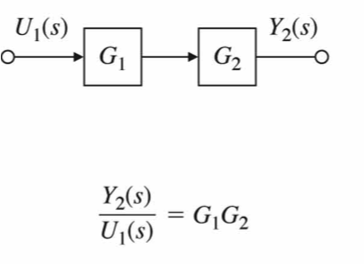
\includegraphics[width=1\textwidth]{images/kettenschaltung}
            \label{fig:kettenschaltung}
            \caption{Kettenschaltung}
        \end{subfigure}%
        \begin{subfigure}{.3\textwidth}
    \centering
    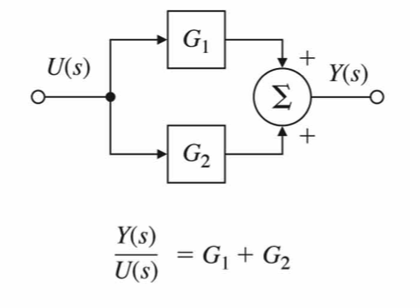
\includegraphics[width=1\textwidth]{images/parallel}
    \caption{Parallelschaltung}
    \label{fig:parallel}
        \end{subfigure}%
            \begin{subfigure}{.3\textwidth}
                \centering
                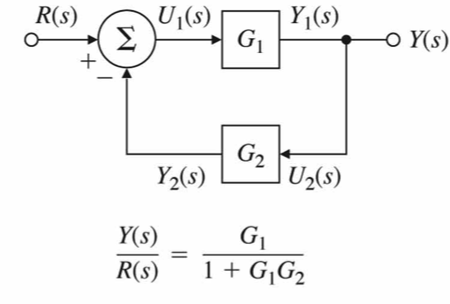
\includegraphics[width=1\textwidth]{images/back}
                \caption{Rückführung}
                \label{fig:back}
            \end{subfigure}%
    \end{figure}
\begin{figure}[H]

            \begin{subfigure}{.5\textwidth}
            \centering
            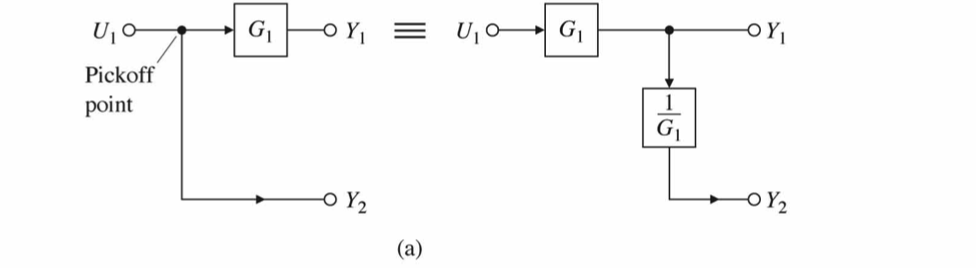
\includegraphics[width=1\textwidth]{images/verschiebung_punkt}
            \caption{Pickoff-Verschiebung}
            \label{fig:pickoff}
            \end{subfigure}%
            \begin{subfigure}{.5\textwidth}
                \centering
                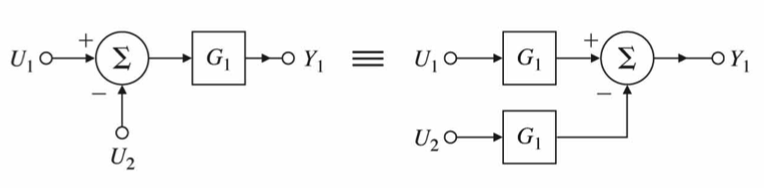
\includegraphics[width=1\textwidth]{images/sum_front}
                \caption{Summationspunkt-Verschiebung}
                \label{fig:sum}
            \end{subfigure}%
            

\end{figure}
\begin{figure}[H]
    \begin{subfigure}{.5\textwidth}
        \centering
        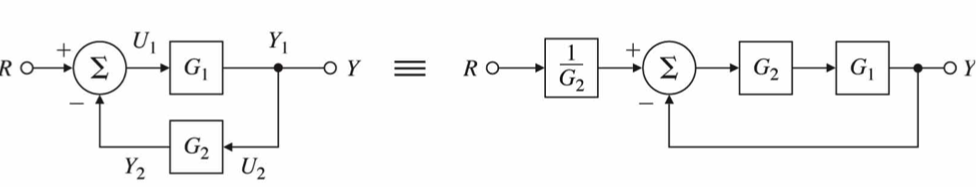
\includegraphics[width=1\textwidth]{images/satz}
        \caption{}
        \label{fig:satz}
    \end{subfigure}%
\end{figure}
\end{tcolorbox}

\begin{tcolorbox}[colback=white!10!white,colframe=gray!50!black,title=Beispiele]
    \begin{figure}[H]
        
        \begin{minipage}{.5\textwidth}
            \centering
            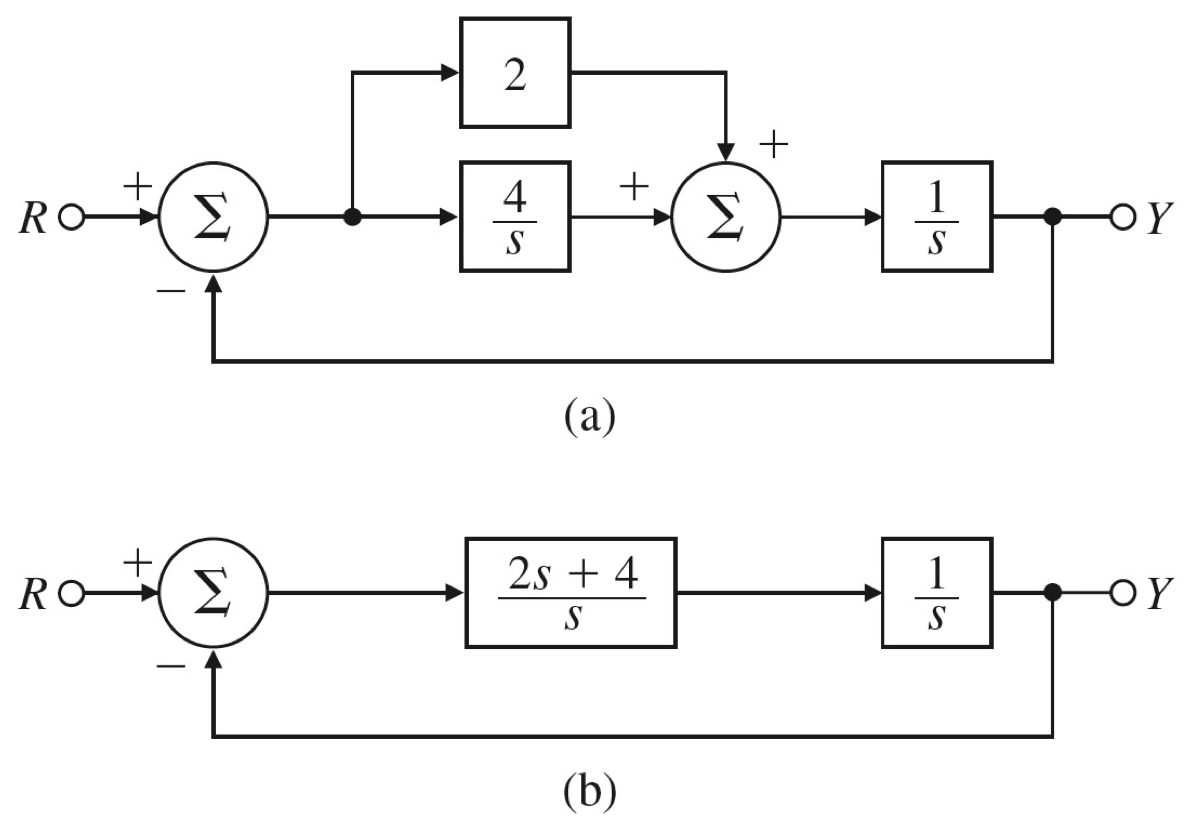
\includegraphics[width=1\textwidth]{images/example_1}
    
        \end{minipage}%
        \begin{minipage}{.5\textwidth}
            \begin{align*}
                T(s) = \frac{\frac{2s+4}{s^2}}{1+\frac{2s+4}{s^2}}
            \end{align*}
        \end{minipage}%
        
        
    \end{figure}
    \begin{figure}[H]
    \noindent\rule[0.2ex]{\linewidth}{1pt}
    
        \begin{minipage}{.5\textwidth}
            \centering
            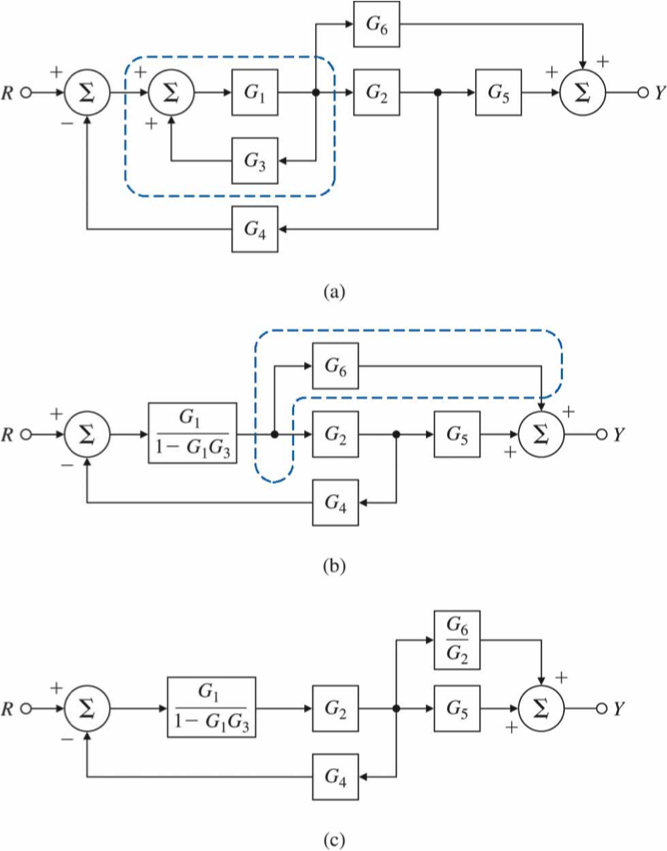
\includegraphics[width=1\textwidth]{images/example_2}
            
        \end{minipage}%
        \begin{minipage}{.5\textwidth}
            \begin{align*}
            &T(s) = \frac{\frac{G_1G_2}{1-G_1G_3}}{1+\frac{G_1G_2G_4}{1-G_1G_3}}\cdot\\& \cdot(G_5+\frac{G_6}{G_2})\\
            &= \frac{G_1G_2G_5+G_1G_6}{1-G_1G_3+G_1G_2G_4}
            \end{align*}
        \end{minipage}%
        
        
    \end{figure}

\end{tcolorbox}
